\documentclass{SBCbookchapter}
\usepackage[utf8]{inputenc}
\usepackage[T1]{fontenc}
\usepackage[brazil,english]{babel}
\usepackage{graphicx}
\title{Comparing Disaster Relief Organizations}
\author{}
\begin{document}
\maketitle

\vspace{.3in}
\begin{minipage}[r]{4.25in}{\small
Coordination among disaster relief organizations is critical for an effective response after a major disaster. An Adaptive Choice-ased Conjoint Analysis is used to measure preferences or organizations in terms of the amount of funding available,  scale of the dissater, need for the organization's services and the type of partnership available on the ground.}
\end{minipage}

\newpage

\section{Introduction}

\begin{figure}[!htpb]
\centering
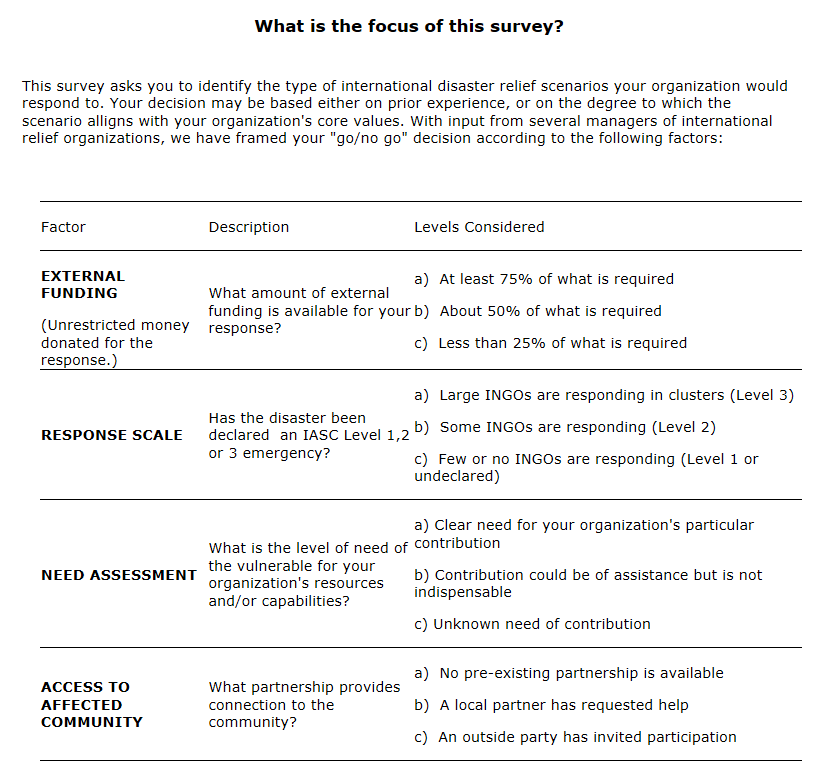
\includegraphics[width=5.75in, height=7in]{AttributeLevels.png}
\caption{{\small An ACBC survey with 4 attributes consisting of 3 levels each. }}
\label{AL}
\end{figure}


\begin{table}[!htpb]
\scriptsize
\centering
\begin{tabular}{c|ccccc|ccccc|ccc|c}
Profile& 1 & 2 & 3 & 4 & 5 & 6&7&8&9&10&11&12&13&PR\\\hline
1212& 2&	3&	7&	3&	7&	7&	1&	7&	7&	7&	4&	1&	7&	4.846\\
1112&7	&1	&7	&7	&1	&2	&7	&5	&7	&3	&7	&7	&4	&5.000\\
1312&7	&7	&7	&7	&5	&5	&7	&1	&1	&1	&7	&7	&3	&5.000\\
3212&7	&7	&7	&5	&5	&1	&2	&7	&4	&7	&7	&7	&1	&5.154\\
1122&1	&7	&7	&4	&7	&7	&5	&7	&4	&7	&3	&3	&7	&5.308\\
2212&7	&5	&5	&7	&7	&7	&7	&2	&7	&4	&2	&2	&7	&5.308\\
1222&7	&7	&4	&7	&4	&5	&7	&4	&3	&2	&7	&7	&7	&5.462\\
1232&5	&7	&7	&5	&5	&5	&4	&5	&7	&5	&7	&7	&2	&5.462\\
2312&7	&7	&7	&1	&5	&3	&4	&7	&2	&7	&7	&7	&7	&5.462\\
2112&3	&7	&7	&4	&5	&4	&3	&7	&7	&7	&7	&7	&5	&5.615\\\hline
\end{tabular}
\caption{{\small Top 10 ranked profiles for FBOs ($n=13,N=50$) }   }
\label{Tab13}
\end{table}

 



\section{Computer Project}
Write a program which can create SBTs for the default and $p$-norm models such as shown in Figure \ref{gucholfig}.





\subsection*{Acknowledgements}

The authors would like to thank
Erica Gralla, Jarrod Goenzel, Timotius Kartawijaya, and Mike Veatch for their valuable contributions to this work.


\section*{References}
\begin{list}{}{\itemindent=-2em}
\small


\item Gralla, E., Goentzel, J., and Fine G. 2014. Assessing trade-offs among multiple objectives for humanitarian aid delivery using expert preferences.
Production and Operations Management, Springer-Verlag Berlin 23(6), 978-989.

\item Orme, B.K., and Chrzan, K. 2017. Becoming an Expert in Conjoint Analysis: Choice Modeling for Pros. Sawtooth Software.

\item Rao, V. R. 2014. Applied Conjoint Analysis. Springer.


\item Rossi, P., Allenby, G. and McCulloch R. 2005. Baysian Statistics and Marketing. John Wiley \& Sons, Ltd.


\end{list}
\end{document}

\emph{Project Team: Danilo Doedrichs, Skyler Laney, Leo O'Malley, Nate Schatz, Cathy Shi, 

\newpage
 \begin{thebibliography}{9}

 \bibitem{Arakawa}  {\sc  ARAKAWA, H.}, 1964. Statistical method to forecast the movement and the central pressure of typhoons in the western north Pacific. \emph{J. Appl. Meteorol.} {\bf 3}, 524-528.

     \bibitem{Cap}   {\sc CAP, F.}, 200.: {\em Tsunamis and Hurricanes: A Mathematical Approach.} Springer-Verlag, 201 pp.

\bibitem{Chan} {\sc CHAN, J.C.L.}, 2005: The physics of tropical cyclone motion. \emph{Annu. Rev. Fluid Mech.} {\bf 37}, 99-128.
\bibitem{Hig}  {\sc HIGAKI, M.}, {\sc KYOUDA, M.} and {\sc YAMAGUCH, H.} 2015. Upgrade of JMA's Typhoon Ensemble Prediction System. http://www.wcrp-climate.org/ WGNE/ Blue Book/2014/individual-articles/06\_Higaki\_Masakazu\_  \\WGNE\_BB2014\_TEPSupgrade\_higaki.pdf



\bibitem{Ito}   {\sc  ITO, K. } and  {\sc WU, C.   }, 2013. \emph{Typhoon-position-oriented sensitivity analysis. part I: theory and verification. } \emph{J. Atmos. Sci.}, {\bf 70}, 2525-2546.

    \bibitem{JMA} {\sc JAPAN METEORLOLOGICAL AGENCY}, 2014: \emph{Annual Report of the RSMC Tokyo-Typhoon Center 2013}. http://www.jma.go.jp/jma/ jma- eng/jma-center/rsmc-hp-pub-eg/AnnualReport/2013/Text/Text2013.pdf

\bibitem{Neumann} {\sc NEUMANN, C. J.}, 1972. \emph{An alternate to the HURRAN tropical cyclone forecast system.} \emph{NOAA Tech. Memo.} NWS SR-62, 22 pp.

\end{thebibliography}

%
\end{document}\documentclass{SBCbookchapter}
\usepackage[utf8]{inputenc}
\usepackage[T1]{fontenc}
\usepackage[brazil,english]{babel}
\usepackage{graphicx}
\title{Face Recognition}
\begin{document}
\maketitle

%\addcontentsline{toc}{chapter}{Statistics}

%\emph{Find a statistical method which uses only Japan Meteorological Agency (JMA) best track typhoon data during or before year $n$ to hind-cast the entire best track of all typhoons in years $n+1$.   Given only the latter typhoons' initial three best track points (i.e. at $t=0,6,$ and $12$ hours), the maximum position error at each hind-casted track point must be less than 500 km. The method must work for the three most recent years of published best track data.}

\vspace{.3in}
\begin{minipage}[r]{4.25in}{\small
  Child trafficking is a heinous crime which should be combatted by all means including advanced technology.  In the case of trans-national
  trafficking, border control may utilize face recognition technology to aid in the rescue of trafficked children.

\newpage

\section{Introduction}


\begin{figure}[h]
\hspace{1.2in} \includegraphics[width=4in, height=2.25in]{HaiyanTrackDefault.png}
 \caption{Default model simulation of Haiyan (2013) which exhibited a 1500 km track error at the 120 hr mark. See Table \ref{typ2}. }
 \centering
 \label{haiyanbasic}
\end{figure}


    \begin{table}[h]
\centering
\tiny
\begin{tabular}{|l|l|l|l|l|l|l|l|l|}
\multicolumn{9}{c}{$p$-NORM MODEL PARAMETERS }\\\hline
&$\Omega_0$ & $\Omega_1$ & $\Omega_2$ & $\Omega_3$ & $\Omega_4$ & $p$ &\multicolumn{2}{l|}{$\gamma$}\\\hline
Latitude &  .5 & 25 & .25 & 59.5 & 0 & 1.3 & \multicolumn{2}{l|}{.05} \\
Longitude &  0 & 0 & 0 & 0 & 0 & 0 & \multicolumn{2}{l|}{.35} \\
Intensity &  .01 & 1 & 10 & 5 & 0 & 1.2 & \multicolumn{2}{l|}{.2} \\
Pressure & .4 &1000&.65&20&5&1.1&\multicolumn{2}{l|}{.6} \\ \hline \hline
\multicolumn{9}{|c|}{POSITION ERRORS }\\\hline
  Hours in advance    & 24-hr & 48-hr &72-hr &96-hr & 120-hr & 144-hr & 168-hr& 192-hr\\\hline
  Default position error  (km)  &297.6  &477.3 & 728.0&1021.9 & 1498.8 &1874.3  & 2105.0 &  1975.6 \\\hline
  $p$-norm position error  (km)   &  125.1  &  97.2  & 46.6  & 65.5  & 167.3& 266.7  &  445.1&   634.6   \\\hline
  Relative error reduction & $R_1=.58 $  &$R_2=.8 $ &$R_3=.94 $ &$R_4=.94 $ &$R_5=.89 $ &$R_6=.86 $  &$R_7=.79 $ &  $R_{7.75} =.68 $   \\ \hline
 \end{tabular}
  \caption{Haiyan (international ID 1330) $p$-norm model simulation. DUIR: JMA grade 5 Philippine landfall (2009 up to Haiyan) }
  \label{typ2}
\end{table}

  \begin{table}[h]
\centering
\tiny
   \begin{tabular}{|l|l|l|l|l|l|l|l|}
\multicolumn{8}{c}{$p$-NORM MODEL PARAMETERS }\\\hline
$p$-norm model parameters&$\Omega_0$ & $\Omega_1$ & $\Omega_2$ & $\Omega_3$ & $\Omega_4$ & $p$ &$\gamma$\\\hline
Latitude &  5 & 9.5 & 20 & .2 & 1 & 1.73 & .26 \\
Longitude &  9 & 25 & 15 & .3 & 0 & .5 & .95 \\
Intensity &  20 & 1 & 10 & 5 & 0 & 1 & .5 \\
Pressure & 1 &10&15&15&12.5&1.1&.85 \\ \hline \hline
\multicolumn{8}{|c|}{POSITION ERRORS }\\\hline
  Hours in advance   & 24-hr & 48-hr &72-hr &96-hr & 120-hr &   144-hr& 168-hr\\\hline
 Default position error  (km)&  15.3  & 140.4    & 31.6  & 198.2   & 203.1 &  341.0 &747.1 \\\hline
 $p$-norm position error  (km)&  37.8  &  150.0  & 162.9  & 416.2  &  390.1& 151.1&159.1 \\\hline
 Relative error reduction & $R_1= -1.47 $  &$R_2=-.07 $ &$R_3=-4.16 $ &$R_4=-1.1 $ &$R_5=-.92 $ &$R_6=.56 $  &$R_7=.79 $ \\ \hline \hline
   Hours in advance   &  192-hr &216-hr & 240-hr &  264-hr & 288-hr &  312-hr & 336-hr \\\hline
 Default position error  (km)    & 1257.1  & 1892.1   & 2722.0 &3343.9  & 4140.6    & 4659.2  & 5088.5     \\\hline
 $p$-norm position error  (km)  & 348.3  & 647.7  &  1096.9&   1284.4  &  1548.0  & 1473.7  & 1126.3       \\\hline
 Relative error reduction & $R_8=.72 $ &$R_9=.66 $ &$R_{10}=.62 $   & $R_{11}=.60 $  &$R_{12}=.62 $ &$R_{13}=.68 $ &$R_{14}=.78$ \\ \hline \hline
 \end{tabular}
  \caption{Guchol (international ID 1204) $p$-norm model simulation. DUIR:  JMA best track grade 5 typhoon data (2009-)}
  \label{typ3}
 \end{table}
\begin{figure}[h]
\centering
  \includegraphics [width=2.5in, height=2.25in]{GucholTrackDefault.eps}
  \includegraphics[width=2.5in, height=2.25in]{GucholTrackp.eps}
     \caption{Missing curvature in the default model of Guchol (2012) is corrected by the $p$-norm model (solid markers=actual, dashed=simulated; parameters given in Table 3.)}
  \label{gucholfig}
\end{figure}



\section{Computer Project}
Write a program which can create SBTs for the default and $p$-norm models such as shown in Figure \ref{gucholfig}.





\vspace{1in}

\emph{Acknowledgement:} Guidance from Dr. Takemasa Miyoshi and the Journal of the Meteorological Society of Japan's editorial staff is gratefully acknowledged. This project was supported by Wheaton College's Summer Research Programs.
.
\vspace{.25in}

\emph{Project Team:} Korey Clement, Daniela Cuba, Michael Kietzman, Peyton Finley, Jacob Clement, Danilo Diedrichs, Roland Hesse, Spencer Hills, Kaile Phelps, Jenny Ruda, Erica Swain, Kei Takazawa, Emily Wilson

\newpage
 \begin{thebibliography}{9}

 \bibitem{Arakawa}  {\sc  ARAKAWA, H.}, 1964. Statistical method to forecast the movement and the central pressure of typhoons in the western north Pacific. \emph{J. Appl. Meteorol.} {\bf 3}, 524-528.

     \bibitem{Cap}   {\sc CAP, F.}, 200.: {\em Tsunamis and Hurricanes: A Mathematical Approach.} Springer-Verlag, 201 pp.

\bibitem{Chan} {\sc CHAN, J.C.L.}, 2005: The physics of tropical cyclone motion. \emph{Annu. Rev. Fluid Mech.} {\bf 37}, 99-128.
\bibitem{Hig}  {\sc HIGAKI, M.}, {\sc KYOUDA, M.} and {\sc YAMAGUCH, H.} 2015. Upgrade of JMA's Typhoon Ensemble Prediction System. http://www.wcrp-climate.org/ WGNE/ Blue Book/2014/individual-articles/06\_Higaki\_Masakazu\_  \\WGNE\_BB2014\_TEPSupgrade\_higaki.pdf



\bibitem{Ito}   {\sc  ITO, K. } and  {\sc WU, C.   }, 2013. \emph{Typhoon-position-oriented sensitivity analysis. part I: theory and verification. } \emph{J. Atmos. Sci.}, {\bf 70}, 2525-2546.

    \bibitem{JMA} {\sc JAPAN METEORLOLOGICAL AGENCY}, 2014: \emph{Annual Report of the RSMC Tokyo-Typhoon Center 2013}. http://www.jma.go.jp/jma/ jma- eng/jma-center/rsmc-hp-pub-eg/AnnualReport/2013/Text/Text2013.pdf

\bibitem{Neumann} {\sc NEUMANN, C. J.}, 1972. \emph{An alternate to the HURRAN tropical cyclone forecast system.} \emph{NOAA Tech. Memo.} NWS SR-62, 22 pp.

\end{thebibliography}

%
\end{document} 